% fig_dt_cycle_budget.tex
% TR-44: DT cycle budget (horizontal stacked bar)
%
% Total = 284.8 µs = 28.5% of 1000 µs budget
% Tasks:
%   EKF update:           17.6 µs (1.8%)
%   Library lookup:      107.2 µs (10.7%)
%   Protection model:     50.0 µs (5.0%)
%   Decision comparison:  10.0 µs (1.0%)
%   GOOSE framing:       100.0 µs (10.0%)
%   Margin:              715.2 µs (71.5%)

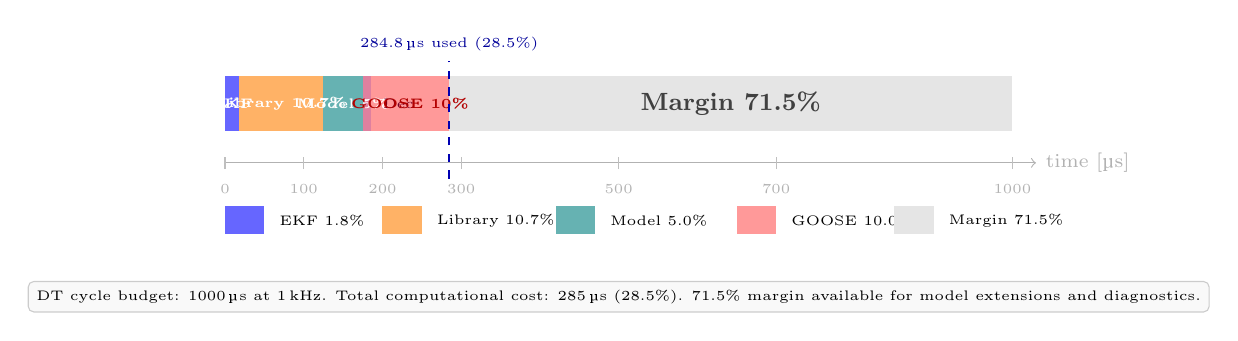
\begin{tikzpicture}[
  every node/.style={font=\scriptsize},
]

\def\bh{0.70}   % bar height
\def\bw{10.0}   % total bar width = 1000 µs

%% Scale: 1 µs → 0.010 cm

%% EKF: 0.176 cm
\fill[blue!60]    (0.000, 0) rectangle (0.176, \bh);

%% Library lookup: 1.072 cm
\fill[orange!60]  (0.176, 0) rectangle (1.248, \bh);

%% Protection model: 0.500 cm
\fill[teal!60]    (1.248, 0) rectangle (1.748, \bh);

%% Decision comparison: 0.100 cm
\fill[purple!50]  (1.748, 0) rectangle (1.848, \bh);

%% GOOSE framing: 1.000 cm
\fill[red!40]     (1.848, 0) rectangle (2.848, \bh);

%% Margin: 7.152 cm
\fill[gray!20]    (2.848, 0) rectangle (10.00, \bh);

%% Labels inside/outside bars
\node[white, font=\tiny\bfseries] at (0.088, 0.35) {EKF};
\node[white, font=\tiny\bfseries] at (0.712, 0.35) {Library 10.7\%};
\node[white, font=\tiny\bfseries] at (1.498, 0.35) {Model 5\%};
\node[purple!60!black, font=\tiny, right=1pt] at (1.848, 0.35) {Dec};
\node[red!70!black, font=\tiny\bfseries] at (2.348, 0.35) {GOOSE 10\%};
\node[gray!50!black, font=\small\bfseries] at (6.424, 0.35) {Margin 71.5\%};

%% Axis
\draw[gray!60, ->] (0, -0.40) -- (10.30, -0.40) node[right] {time [µs]};
\foreach \x/\lab in {0/0, 1/100, 2/200, 3/300, 5/500, 7/700, 10/1000}{
  \draw[gray!50, thin] (\x, -0.48) -- (\x, -0.32);
  \node[gray!60, below=2pt, font=\tiny] at (\x, -0.48) {\lab};
}

%% Total used marker
\draw[blue!70!black, thick, dashed]
  (2.848, -0.60) -- (2.848, \bh + 0.20);
\node[blue!60!black, font=\tiny, above] at (2.848, \bh + 0.20)
  {284.8\,µs used (28.5\%)};

%% Legend row
\def\ly{-1.30}
\fill[blue!60]   (0.0, \ly) rectangle (0.5, \ly+0.35);
\node[right=2pt, font=\tiny] at (0.5, \ly+0.17) {EKF 1.8\%};
\fill[orange!60] (2.0, \ly) rectangle (2.5, \ly+0.35);
\node[right=2pt, font=\tiny] at (2.5, \ly+0.17) {Library 10.7\%};
\fill[teal!60]   (4.2, \ly) rectangle (4.7, \ly+0.35);
\node[right=2pt, font=\tiny] at (4.7, \ly+0.17) {Model 5.0\%};
\fill[red!40]    (6.5, \ly) rectangle (7.0, \ly+0.35);
\node[right=2pt, font=\tiny] at (7.0, \ly+0.17) {GOOSE 10.0\%};
\fill[gray!20]   (8.5, \ly) rectangle (9.0, \ly+0.35);
\node[right=2pt, font=\tiny] at (9.0, \ly+0.17) {Margin 71.5\%};

%% Caption note
\node[draw=gray!40, fill=gray!5, rounded corners=2pt,
      font=\tiny, inner sep=3pt, align=center]
  at (5.0, -2.10)
  {DT cycle budget: 1000\,µs at 1\,kHz. Total computational cost: 285\,µs (28.5\%).
   71.5\% margin available for model extensions and diagnostics.};

\end{tikzpicture}
